\PassOptionsToPackage{obeyspaces,spaces}{url}
\documentclass[10pt,a4paper]{article}

\usepackage[a4paper,margin=1.8cm,top=1.6cm,bottom=1.8cm]{geometry}
% Compiles with XeLaTeX/Tectonic (fontspec) or pdfLaTeX (Type 1 fonts)
\usepackage{iftex}
\ifTUTeX
  \usepackage{newtxtext,newtxmath}
  \setmonofont{Inconsolatazi4}[Extension=.otf,UprightFont=*-Regular,BoldFont=*-Bold,Scale=0.9]
\else
  \usepackage[T1]{fontenc}
  \usepackage{newtxtext,newtxmath}
  \usepackage[scale=0.9,varqu]{inconsolata}
\fi
\usepackage{microtype}
\usepackage{pgfplots}
\pgfplotsset{compat=1.17}
\usepackage{amsmath}
\usepackage{booktabs}
\usepackage{tabularx}
\usepackage{multirow}
\usepackage{enumitem}
\usepackage{xcolor}
\usepackage{tikz}
\usetikzlibrary{positioning,arrows.meta,fit,backgrounds}
\usepackage{titlesec}
\usepackage[font=small,labelfont=bf,skip=3pt]{caption}
\usepackage{fancyhdr}
\usepackage[hidelinks]{hyperref}

\titleformat{\section}{\large\bfseries}{\thesection.}{0.5em}{}
\titlespacing*{\section}{0pt}{8pt}{3pt}
\titleformat{\subsection}[runin]{\normalsize\bfseries}{}{0pt}{}[.]
\titlespacing*{\subsection}{0pt}{4pt}{0.6em}
\setlist{nosep,leftmargin=1.3em}
\setlength{\parskip}{2pt}
\setlength{\parindent}{0pt}
\emergencystretch=1.5em

% inline code: monospace, may break after _ . , ( and at spaces
\usepackage{url}
\DeclareUrlCommand\code{\urlstyle{tt}}
\renewcommand{\UrlBreaks}{\do\_\do\.\do\,\do\(\do\/}
\definecolor{accent}{HTML}{1F4E79}
\definecolor{soft}{HTML}{EEF3F8}

\pagestyle{fancy}
\fancyhf{}
\renewcommand{\headrulewidth}{0pt}
\fancyfoot[L]{\footnotesize CS631 Final Report: Distributed GSI Maintenance for Sharded PostgreSQL}
\fancyfoot[R]{\footnotesize\thepage}

\begin{document}

\begin{center}
{\LARGE\bfseries Distributed GSI Maintenance for Sharded PostgreSQL}\\[3pt]
{\large Final Report, CS631 Course Project, IIT Bombay}\\[4pt]
Kunj Bhesaniya (23B0995) \textperiodcentered{} Dhruvraj Merchant (23B1041) \textperiodcentered{}
Dipen Sojitra (23B0913) \textperiodcentered{} Harshil Solanki (23B1016)
\end{center}
\vspace{-4pt}

%=====================================================================
\section{Introduction}

When a table is sharded across PostgreSQL servers by its primary key, a query on another column
(\code{WHERE email = ?}) must be sent to every shard, and \code{UNIQUE(email)} cannot be enforced
because each shard sees only its own rows. Spanner, CockroachDB and TiDB solve this with a
\emph{global secondary index} (GSI); core PostgreSQL has none. We built one as a PostgreSQL~16 C
extension, \textbf{\code{gsi_fdw}}, a modified copy of \code{postgres_fdw}. The index entry for key
$k$ lives on node $\mathrm{hash}(k) \bmod N$, independent of where the row lives, so every write
touches two nodes and the core problem is keeping table and index consistent under concurrent
writes and crashes.

\textbf{What changed since Checkpoint~1.} The checkpoint had the catalog, a GSI read path with a
fixed cost, synchronous maintenance with two-phase commit (2PC) and a crash resolver.
Table~\ref{tab:plan} maps the next steps we listed there to what we built. We also made hop~2 of
the read parallel, and added a live demo with 2PC tracing and fault injection.

\begin{table}[h]
\centering\small
\caption{Checkpoint~1 next steps and their status in the final system.}
\label{tab:plan}
\begin{tabularx}{\linewidth}{@{}>{\hsize=.75\hsize}X>{\hsize=1.25\hsize}Xl@{}}
\toprule
Checkpoint~1 plan & Final system & Section \\
\midrule
Benchmarks with and without the GSI & 7 experiments: lookups, writes, node count, hot keys, async lag, build, TPC-C & \S8 \\
Selectivity-based cost model & expected entries $k$ from statistics, expected shards $S(k)$, per-hop cost & \S3 \\
Online index build (\code{gsi_create} worked only on empty tables) & \code{CALL gsi_create} on populated tables while writes continue; resumable & \S6 \\
Asynchronous mode, measure the lag & per-shard outbox, applier workers, \code{gsi_lag()} & \S7, \S8 \\
Sharding without hard-coding / more schemas & any table hash-partitioned by one column of any type; e.g.\ a TPC-C \code{customer} table & \S2, \S8 \\
\bottomrule
\end{tabularx}
\vspace{-6pt}
\end{table}

%=====================================================================
\section{Setup: Docker cluster and PostgreSQL nodes}

\begin{figure}[!ht]
\centering
\begin{tikzpicture}[
  font=\footnotesize,
  box/.style={draw=accent,rounded corners=2pt,fill=white,align=center,inner sep=3pt},
  comp/.style={draw=accent!60,fill=soft,rounded corners=1pt,align=center,inner sep=2pt,font=\scriptsize},
  arr/.style={-{Stealth[length=4pt]},thick,accent},
  darr/.style={-{Stealth[length=4pt]},thick,dashed,orange!80!black}]
  % coordinator
  \node[comp] (planner) at (0,0) {planner hook\\\code{GsiLookup} scan};
  \node[comp,right=3pt of planner] (fdw) {FDW modify hooks\\index maintenance};
  \node[comp,right=3pt of fdw] (tpc) {xact callback\\2PC};
  \node[comp,right=3pt of tpc] (bg) {bg workers:\\resolver, appliers};
  \node[comp,right=3pt of bg] (cat) {catalog \code{gsi.*}\\\code{users} (partitioned)};
  \begin{scope}[on background layer]
  \node[box,fit=(planner)(cat),inner sep=4pt,label={[font=\footnotesize\bfseries,anchor=south west]north west:coordinator (port 5432)}] (coord) {};
  \end{scope}
  % shards
  \foreach \i/\x in {1/-0.4,2/3.0,3/6.4,4/9.8,5/13.2}{
    \node[box,minimum width=2.9cm] (s\i) at (\x,-1.75)
      {\textbf{shard\i} (node \the\numexpr\i-1\relax)\\[-1pt]
       {\scriptsize\code{users_shard} (base rows)}\\[-1pt]
       {\scriptsize\code{gsi_users_email} slice}\\[-1pt]
       {\scriptsize\code{gsi_outbox}}};
  }
  \draw[arr] (planner.south) -- node[left,font=\scriptsize,pos=0.45]{hop 1} (s1.north);
  \draw[arr] (planner.south east) -- node[right,font=\scriptsize,pos=0.6]{hop 2} (s2.north);
  \draw[darr] (fdw.south) -- (s3.north);
  \draw[darr] (tpc.south) -- node[right,font=\scriptsize,pos=0.55]{PREPARE / COMMIT PREPARED} (s4.north);
\end{tikzpicture}
\caption{Cluster layout. Every data node holds one base partition, its slice of every GSI table,
and an outbox for async GSIs. A read asks one index node (hop~1), then only the shards that hold
matching rows (hop~2).}
\label{fig:arch}
\vspace{-6pt}
\end{figure}

\textbf{Cluster.} \code{docker/docker-compose.yml} starts one coordinator and five data nodes
(\code{shard1..5}) from one image (\code{postgres:16-bookworm} plus our extension, built by the
\code{Dockerfile}). \code{NNODES=2..5} selects how many nodes are used. Data nodes run with
\code{max_prepared_transactions=100}; the coordinator also preloads \code{gsi_fdw} so its
background workers start. \code{bench/net_delay.sh} adds a round-trip delay between containers
with \code{tc netem}, so a hop costs what it would between machines.

\textbf{Sharding.} \code{init/coordinator.sh} creates one foreign server per node, lists the nodes
in \code{gsi.gsi_node(node_id, server_name)}, and creates \code{users(id, email, name)}
\code{PARTITION BY HASH (id)} whose partitions are foreign tables on the shards. PostgreSQL's own
tuple routing sends each row to its shard. Servers use \code{use_remote_estimate}, so the planner
asks each shard for the real cost of the broadcast plan (including shard-local indexes).

\textbf{GSI catalog and layout.} \code{gsi.gsi_index} has one row per GSI: base table, column,
\code{is_unique}, \code{mode} (\code{sync}/\code{async}) and \code{status}
(\code{write-only}/\code{ready}). Each node holds a table \code{gsi_<table>_<col>(key, id, shard)}
with primary key \code{(key, id)}, plus a unique index on \code{key} for a unique GSI. An entry
stores the indexed value, the row identifier and the node that holds the row, so a lookup fetches
from exactly the right shard and an UPDATE/DELETE removes exactly that row's entry. Placement uses
the type's extended hash with PostgreSQL's hash-partitioning seed, mod $N$
(\code{gsi_node_for_datum}); every component (writes, reads, build, applier, checker) uses this one
function. The \textbf{row identifier} is the table's partition-key column, of any name and type
with a B-tree ordering; \code{gsi_create} checks that every shard has a unique, non-partial index
on it and that it is \code{NOT NULL}, so per-shard uniqueness is global uniqueness.

\textbf{Code.} About 3{,}300 new lines of C: \code{gsi.c} (catalog, placement, write maintenance),
\code{gsi_scan.c} (planner hook, cost model, \code{GsiLookup}), \code{connection.c} (+267 lines,
2PC), \code{gsi_resolver.c}, \code{gsi_build.c} (online build), \code{gsi_async.c} (outbox
appliers), and 32 lines of hooks in \code{postgres_fdw.c}.

%=====================================================================
\section{Read path: plan, cost and execution}

\subsection{Plan}
A \code{set_rel_pathlist_hook} looks at every \code{SELECT} on a partitioned table (not a write
target, no row locks) for a qual \code{col = Const} or \code{col = $n} using the type's default
equality operator, on a column with a \code{ready} GSI. If several match it prefers a unique GSI.
It adds a \code{GsiLookup} CustomPath next to PostgreSQL's Append over all partitions; the cheaper
one wins. Parameters are supported, so prepared statements and generic plans use the GSI too.

\subsection{Cost}
For a lookup expected to match $k$ entries on $N$ nodes:
\vspace{-3pt}
\begin{align*}
S &= N\bigl(1-(1-1/N)^{k}\bigr) \quad\text{(expected shards holding the $k$ rows; rows are placed by hash(id))}\\
\text{Cost} &= \underbrace{c_{rt} + c_{probe}\lceil k/e\rceil + k\,c_{tup}}_{\text{hop 1: one index node}}
 \;+\; \underbrace{S\,c_{rt} + k\,c_{probe} + k\,c_{tup}}_{\text{hop 2: PK probes on $S$ shards}}
 \;+\; \underbrace{k\,c_{qual}}_{\text{recheck}}
\end{align*}
\vspace{-12pt}

where $c_{rt}$ is the cost of one remote query (\code{fdw_startup_cost}), $c_{tup}$ the cost of
shipping a row, $c_{probe}$ one index probe (a random page read plus CPU costs), and $e$ the
entries per index page. These are the constants \code{postgres_fdw} uses for the Append it competes with. $k=1$ for a
unique GSI; otherwise $k$ is the equality selectivity from the table's inherited statistics times
its row count (\code{gsi_create} runs \code{ANALYZE} when the index becomes ready).

\subsection{Execution}
Hop~1 hashes the runtime key and runs \code{SELECT id, shard FROM gsi_... WHERE key = $1} on that
one node. Hop~2 groups the returned ids by shard and sends \code{... WHERE id = ANY($1)} to only
those shards; all queries are sent before any result is read, so hop~2 costs about one round trip
instead of one per shard (our first version was sequential). Every original qual is
\textbf{rechecked} on the fetched rows, so a stale or uncommitted entry can never produce a wrong
row. \code{EXPLAIN} shows the chosen GSI and estimated entries and shards, and \code{EXPLAIN ANALYZE}
adds the index node and shards actually fetched. \code{gsi.enable_lookup} and
\code{gsi.force_lookup} disable or force the path for experiments.

%=====================================================================
\section{Write path: index maintenance}

Every INSERT, UPDATE and DELETE changes the base row and its entry in every GSI of the table in the
same distributed transaction:
\begin{enumerate}
\item \textbf{No pushdown.} If a statement can change an entry (INSERT, DELETE, UPDATE of an
indexed column), our check in the direct-modify planner refuses the whole-statement pushdown and the
batch size is forced to 1, so our per-row hooks run. An UPDATE that sets no indexed column keeps
\code{postgres_fdw}'s pushdown and its normal commit.
\item \textbf{Old values.} \code{AddForeignUpdateTargets} adds junk columns with the old key of
every GSI and the old row id, so we know which entries to delete.
\item \textbf{Capture, write, apply.} Before the base write we compute the old and new entries
(the RETURNING slot is overwritten afterwards). After the base write succeeds we run
\code{DELETE ... WHERE key = $1 AND id = $2} on the old key's node and \code{INSERT (key, id,
shard)} on the new key's node, on \code{postgres_fdw}'s cached connections, so both join the same
remote transactions. An UPDATE that leaves the key unchanged touches no entry; a NULL key has no
entry. Values travel as text under \code{postgres_fdw}'s transmission settings, so keys of any
type (dates, floats, uuid) round-trip exactly.
\item \textbf{Conflicts.} If the delete removes no row, a concurrent transaction changed that entry
since our snapshot; we raise a serialization failure and the client retries.
\item \textbf{Uniqueness.} A unique GSI has a unique B-tree on \code{key} on the index node. Two
rows with the same email, even on different shards, send their entries to the same node, so the
second insert waits for the first and fails if it commits.
\end{enumerate}
Changing the partition key is rejected (foreign partitions cannot move a row between shards).

%=====================================================================
\section{Two-phase commit and recovery}

Any transaction that wrote a sync GSI commits all its remote transactions with 2PC, inside
\code{postgres_fdw}'s transaction callback:
\begin{enumerate}
\item \textbf{Make the xid durable.} A transaction that only wrote remotely has no local WAL record,
so after a crash its xid could be reused and a later commit misread as its decision. We assign the
full xid and write and flush a small WAL message first.
\item \textbf{Prepare} (pre-commit): \code{PREPARE TRANSACTION 'gsi_<fxid>_<server>_<i|b>'} on every
participant (\code{i} = wrote an index entry, \code{b} = base only). Any failure raises an error,
the transaction aborts, and every prepared participant is rolled back.
\item \textbf{Decision}: the coordinator's own local commit record for \code{fxid}.
\item \textbf{Commit}: \code{COMMIT PREPARED} on \code{i} participants first, then \code{b}, so a
visible base row always has its index entry. After the decision nothing may throw; a failure is
logged and left to the resolver.
\end{enumerate}

\textbf{Resolver.} \code{gsi_resolve(grace)} and a background worker (every 5\,s, for prepared
transactions older than 10\,s) read \code{pg_prepared_xacts} on every node, parse the \code{fxid}
from each \code{gsi_*} gid, and ask the coordinator \code{pg_xact_status(fxid)}:
\emph{committed} $\to$ \code{COMMIT PREPARED} (index participants first), \emph{aborted} $\to$
\code{ROLLBACK PREPARED}, \emph{in progress} $\to$ leave it to its owner. The resolver only reads
the recorded decision, so it can never disagree with the original transaction.

\textbf{Deadlocks and testing.} Nodes cannot see each other's lock waits, so remote sessions set a
lock timeout (5\,s, \code{gsi.remote_lock_timeout}) and the client retries. For testing,
\code{gsi.fail_point} calls \code{abort()} in the coordinator backend at a named step (a real crash
and crash recovery), \code{gsi.pause_point} stops there so a node can be killed by hand, and
\code{gsi.trace} prints each 2PC step. Figure~\ref{fig:2pc} shows one INSERT with the fail points,
and Table~\ref{tab:crash} the crash scenarios we exercise.

\begin{figure}[!ht]
\centering
\begin{tikzpicture}[font=\scriptsize,
  lane/.style={draw=gray!60,thick},
  msg/.style={-{Stealth[length=3.5pt]},thick,accent},
  cmsg/.style={-{Stealth[length=3.5pt]},thick,green!45!black},
  fp/.style={draw=red!70!black,fill=red!8,rounded corners=1pt,inner sep=1.5pt,font=\scriptsize,text=red!70!black}]
  \foreach \y/\n in {0/coordinator,-1.15/index node,-2.3/base node}{
    \draw[lane] (0,\y) -- (15.3,\y);
    \node[anchor=east,font=\scriptsize\bfseries,align=right] at (0,\y) {\n};
  }
  \draw[msg] (0.45,0) -- (0.45,-2.3); \node[anchor=south,align=center] at (0.45,0) {INSERT\\row};
  \draw[msg] (1.6,0) -- (1.6,-1.15);  \node[anchor=south,align=center] at (1.6,0) {INSERT\\entry};
  \node[draw=accent,fill=soft,inner sep=1.5pt,align=center] at (3.05,0) {COMMIT:\\flush xid};
  \draw[msg] (5.0,0) -- (5.0,-1.15);  \node[anchor=south,align=center] at (5.0,0) {PREPARE\\\code{gsi_X_shard3_i}};
  \draw[msg] (7.3,0) -- (7.3,-2.3);   \node[anchor=south,align=center] at (7.3,0) {PREPARE\\\code{gsi_X_shard2_b}};
  \node[fp] at (8.55,-0.58) {\code{after_prepare}};
  \node[draw=accent,fill=accent,text=white,inner sep=2pt,align=center,font=\scriptsize\bfseries] at (9.75,0) {local commit\\= decision};
  \node[fp] at (11.15,-0.58) {\code{after_local_commit}};
  \draw[cmsg] (12.45,0) -- (12.45,-1.15); \node[anchor=south,align=center] at (12.45,0) {COMMIT\\PREPARED \code{_i}};
  \node[fp] at (13.4,-1.73) {\code{mid_commit_prepared}};
  \draw[cmsg] (14.6,0) -- (14.6,-2.3);  \node[anchor=south,align=center] at (14.6,0) {COMMIT\\PREPARED \code{_b}};
  \draw[thick,gray,-{Stealth[length=3.5pt]}] (0.2,-2.65) -- (15.3,-2.65) node[midway,below,font=\scriptsize,text=gray!30!black]
    {time \quad (red boxes: \code{gsi.fail_point} crash points; X = the coordinator's full xid)};
\end{tikzpicture}
\caption{One INSERT into \texttt{users} with a sync GSI, here with the entry on shard3 (node
$\mathrm{hash}(\text{email}) \bmod N$) and the row on shard2 (node $\mathrm{hash}(\text{id}) \bmod
N$). Both prepare; after the coordinator's local commit, the index participant commits first and
the base participant last.}
\label{fig:2pc}
\vspace{-4pt}
\end{figure}

\begin{table}[!ht]
\centering\small
\caption{Crash scenarios (from our demo) and how they end.}
\label{tab:crash}
\begin{tabularx}{\linewidth}{@{}>{\hsize=.85\hsize}X>{\hsize=1.15\hsize}X@{}}
\toprule
Failure & Outcome \\
\midrule
Data node killed before it prepared & PREPARE fails; the whole transaction rolls back on every node \\
Data node killed after it prepared & prepared transaction survives the node's restart; resolver commits it \\
Coordinator crash at \code{after_prepare} & no commit record $\Rightarrow$ resolver rolls back every participant \\
Coordinator crash at \code{after_local_commit} & committed $\Rightarrow$ resolver rolls forward, index nodes first \\
Coordinator crash at \code{mid_commit_prepared} & entry visible, row still prepared: lookup returns 0 rows (never a wrong row) until resolved \\
\bottomrule
\end{tabularx}
\vspace{-6pt}
\end{table}

%=====================================================================
\section{Online index build}

\code{CALL gsi_create(table, col, unique, mode)} builds a GSI on a populated table without blocking
reads or writes, in the spirit of \code{CREATE INDEX CONCURRENTLY}. It is a procedure because each
step commits before the next:
\begin{enumerate}
\item \textbf{Write-only.} Create the index tables on every node and commit; then insert the catalog
row with status \code{write-only} and invalidate cached plans. From now on every write maintains
the index, but the planner ignores it. (The tables are committed first because the coordinator
commits before the nodes do, so a writer could otherwise see the catalog row before the table.)
The catalog is read with the latest snapshot, so even a \code{REPEATABLE READ} writer sees the new
index.
\item \textbf{Wait for old writers.} \code{WaitForLockers} waits for every transaction that may have
planned its write before step~1. Since every write goes through the one coordinator, every row is
now either written by a writer that knows the index, or visible to the backfill.
\item \textbf{Backfill in chunks.} Per node, rows in id order, \code{gsi.build_chunk_size} at a time
(default 10{,}000), read \code{FOR SHARE} so a concurrent UPDATE/DELETE of them waits and then fixes
the entry itself. Entries go to each index node in one \code{INSERT ... SELECT unnest(...)}
\code{ON CONFLICT DO NOTHING} (skipping entries concurrent writers already made). Each chunk is one
2PC transaction that also records the last id in \code{gsi.gsi_build_progress}, so calling
\code{gsi_create} again after a crash \textbf{resumes}. Conflicts retry the chunk; a duplicate key
in a unique build drops the index and reports the error.
\item \textbf{Validate.} Briefly holding a lock that makes new writes wait (reads continue), compare
count and sum of 64-bit hashes of \code{key:id:shard} computed from the base rows and from the
entries, on every node. For an async GSI the outbox is drained first.
\item \textbf{Ready.} Set status \code{ready}, invalidate plans, \code{ANALYZE} the table.
\end{enumerate}

%=====================================================================
\section{Asynchronous GSIs}

A sync GSI makes every write a multi-node 2PC. With \code{mode => 'async'} a write instead adds one
row \code{(index, old_key, new_key, id)} per GSI to \code{gsi_outbox} on the \emph{base} node, in the
base write's own transaction. A write that touches one node therefore commits in one phase, with no
2PC; 2PC is used only if the transaction touches several nodes.

\textbf{Appliers.} \code{gsi.applier_workers} background workers on the coordinator drain the
outboxes (worker $i$ owns nodes $i, i{+}n, \dots$). Each pass reads up to 1{,}000 rows in
\code{seq} order, applies them on each touched index node in one local transaction (delete the
old entry, insert the new one \code{ON CONFLICT DO NOTHING}), commits, and then deletes exactly
the outbox rows it read. Ordering by \code{seq} is enough because all changes of one row happen on
its base node under its row lock. Deleting the rows read (not \code{seq <= max}) never skips a row
whose smaller \code{seq} committed late, and a crash before the delete just replays the batch,
which gives the same result.

\textbf{Trade-offs.} Reads of an async GSI may miss very recent writes (the recheck still
prevents wrong rows); \code{gsi_lag()} reports pending rows and the age of the oldest per node. A
unique GSI must be sync, since an async one would see a duplicate only after both rows committed.

%=====================================================================
\section{Results}

All six containers run on one machine under Docker Desktop, 5 nodes unless stated. Lookups and the
build use 1M \code{users} rows loaded through the real write path (base row, entries, 2PC); the
write experiments start from an empty table. Latency is per statement, measured by the
client; plans are prepared so planning is not timed. Speedups are against the broadcast plan
(Append over all shards) in the same run. Each write experiment ends with our consistency checker
(missing, orphaned or misplaced entries, leftover prepared transactions).

\textbf{Lookups} (Table~\ref{tab:lookups}). Names are generated so each matches exactly $K$ rows.
Without shard-local indexes broadcast scans every shard, and the GSI is 13--36$\times$ faster. The
fair baseline gives every shard its own index on the column: then the GSI wins by 2.2$\times$ for a
unique key and 1.2--1.5$\times$ for $K \ge 10$, and with a 1\,ms round trip between containers by
1.9--3.8$\times$, because broadcast pays a round trip to every shard. The benefit grows with the
number of nodes: unique-key speedup over the indexed baseline is 1.17$\times$ on 2 nodes,
1.52$\times$ on 3 and 2.23$\times$ on 5, with the GSI flat at about 1.6\,ms. Making hop~2 parallel
cut $K=1000$ lookups from 7.1 to 5.2\,ms (25.5 to 17.6\,ms at 1\,ms RTT).

\begin{figure}[!ht]
\centering
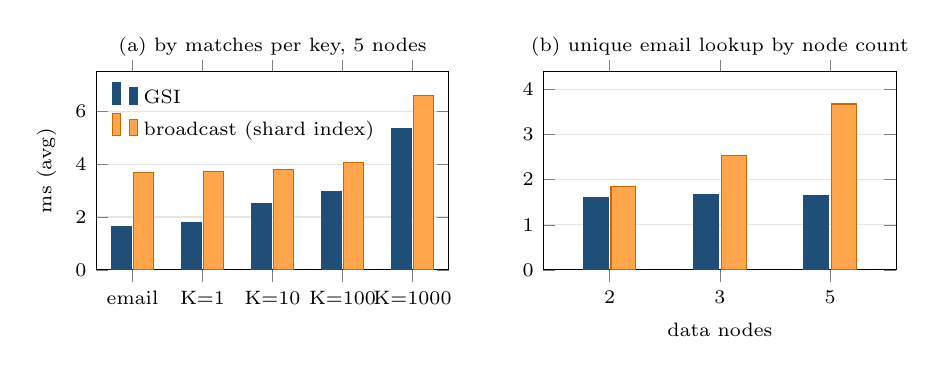
\begin{tikzpicture}
\begin{axis}[name=left, width=0.5\linewidth, height=4.1cm, ybar=1pt, bar width=7pt,
  symbolic x coords={email,K=1,K=10,K=100,K=1000}, xtick=data,
  ylabel={ms (avg)}, ymin=0, ymax=7.5, enlarge x limits=0.13,
  tick label style={font=\scriptsize}, label style={font=\scriptsize},
  title={\scriptsize (a) by matches per key, 5 nodes}, title style={yshift=-4pt},
  legend style={font=\scriptsize,at={(0.02,0.98)},anchor=north west,draw=none,fill=none},
  legend cell align=left, ymajorgrids, grid style={gray!20}]
\addplot[fill=accent,draw=accent] coordinates {(email,1.65) (K=1,1.80) (K=10,2.51) (K=100,2.96) (K=1000,5.34)};
\addplot[fill=orange!70,draw=orange!80!black] coordinates {(email,3.68) (K=1,3.72) (K=10,3.78) (K=100,4.07) (K=1000,6.60)};
\legend{GSI, broadcast (shard index)}
\end{axis}
\begin{axis}[at={(left.east)}, anchor=west, xshift=1.2cm, width=0.5\linewidth, height=4.1cm,
  symbolic x coords={2,3,5}, xtick=data, ybar=1pt, bar width=9pt,
  xlabel={data nodes}, ymin=0, ymax=4.4, enlarge x limits=0.3,
  tick label style={font=\scriptsize}, label style={font=\scriptsize},
  title={\scriptsize (b) unique email lookup by node count}, title style={yshift=-4pt},
  ymajorgrids, grid style={gray!20}]
\addplot[fill=accent,draw=accent] coordinates {(2,1.60) (3,1.67) (5,1.65)};
\addplot[fill=orange!70,draw=orange!80!black] coordinates {(2,1.86) (3,2.54) (5,3.68)};
\end{axis}
\end{tikzpicture}
\vspace{-4pt}
\caption{Lookup latency against the fair baseline (every shard has its own index on the column), no
added network delay. Broadcast grows with the number of shards; the GSI asks one index node and only
the shards that hold matches.}
\label{fig:lookups}
\vspace{-6pt}
\end{figure}

\begin{table}[h]
\centering\small
\caption{Lookup latency (ms, average), 5 nodes, 1M rows. $\hat k$ = entries the cost model expected.
Planner = plan chosen with shard-local indexes present (\checkmark{} = it was the faster one).}
\label{tab:lookups}
\begin{tabular}{@{}lr r rr rr l rr@{}}
\toprule
& & & \multicolumn{2}{c}{broadcast, no shard index} & \multicolumn{2}{c}{broadcast, shard index} & & \multicolumn{2}{c}{1\,ms RTT, shard index}\\
\cmidrule(lr){4-5}\cmidrule(lr){6-7}\cmidrule(l){9-10}
Key & $\hat k$ & GSI & ms & speedup & ms & speedup & Planner & GSI / bcast & speedup \\
\midrule
email (unique) & 1 & 1.65 & 59.5 & 36.3$\times$ & 3.68 & 2.23$\times$ & GSI \checkmark & 8.5 / 32.5 & 3.82$\times$ \\
$K=1$    & 2   & 1.80 & 59.5 & 34.8$\times$ & 3.72 & 2.07$\times$ & GSI \checkmark & 8.5 / 32.6 & 3.84$\times$ \\
$K=10$   & 2.8 & 2.51 & 64.8 & 26.4$\times$ & 3.78 & 1.51$\times$ & GSI \checkmark & 15.3 / 33.0 & 2.15$\times$ \\
$K=100$  & 100 & 2.96 & 64.6 & 22.3$\times$ & 4.07 & 1.37$\times$ & bcast $\times$ & 17.0 / 33.1 & 1.94$\times$ \\
$K=1000$ & 1000 & 5.34 & 66.0 & 12.8$\times$ & 6.60 & 1.24$\times$ & bcast $\times$ & 17.7 / 41.7 & 2.35$\times$ \\
\bottomrule
\end{tabular}
\vspace{-4pt}
\end{table}

\textbf{Cost model.} The planner picks the faster plan in 9 of 10 cases on 2 nodes and 8 of 10 on
3 and 5 nodes. Every miss is at $K \ge 100$, where both plans touch every shard: the planner keeps
broadcast although the GSI is faster. The model still charges hop~2 as $S$ separate round trips
($S\,c_{rt}$), which was right for our first, sequential hop~2 but overprices it now that the
queries run concurrently; at 1\,ms RTT this miss costs about 2$\times$ (17 vs.\ 33\,ms).
\code{use_remote_estimate} itself costs planning time (2.9 vs.\ 2.0\,ms average, p99 25\,ms, on
5 nodes; 15.8\,ms average at 1\,ms RTT), which is why we use prepared statements.

\textbf{Writes} (Table~\ref{tab:writes}). A sync GSI turns each write into a 2PC across 2--3 nodes
with several synchronous disk flushes, so insert throughput drops from 1{,}158 to 177 tps with
one GSI and 114 with two. An async GSI keeps single-node writes one-phase: 605 tps (52\% of no
GSI, 3.4$\times$ sync), and the outbox drains within 0.3\,s after the run. Run-to-run variance on
this setup is large (an earlier run measured 2{,}148 tps with no GSI), so we compare configurations
only within one run.

\begin{table}[h]
\centering\small
\begin{minipage}[t]{0.49\linewidth}\centering
\caption{Write cost (tps / average ms).}
\label{tab:writes}
\begin{tabular}{@{}lrr@{}}
\toprule
GSIs on \code{users} & insert & key update \\
\midrule
none     & 1158 / 6.9 & 759 / 10.5 \\
1 sync   & 177 / 45.3 & 131 / 61.1 \\
2 sync   & 114 / 70.4 & 136 / 58.8 \\
1 async  & 605 / 13.2 & 585 / 13.7 \\
2 async  & 587 / 13.8 & 479 / 16.7 \\
\bottomrule
\end{tabular}
\end{minipage}\hfill
\begin{minipage}[t]{0.49\linewidth}\centering
\caption{Async lag: outbox age and how soon a just-inserted row is found through the GSI (ms).}
\label{tab:lag}
\begin{tabular}{@{}rrrrr@{}}
\toprule
writers & tps & lag p50 / p99 & visible p50 / p99 \\
\midrule
1  & 312  & 89 / 120  & 56 / 112 \\
4  & 1230 & 111 / 126 & 67 / 126 \\
8  & 788  & 175 / 298 & 95 / 194 \\
16 & 1057 & 232 / 375 & 119 / 254 \\
\bottomrule
\end{tabular}
\end{minipage}
\vspace{-4pt}
\end{table}

\textbf{Async lag} (Table~\ref{tab:lag}). A lookup issued right after the insert misses the row in
99--100\% of probes; it becomes visible after 56--119\,ms at the median and at most 254\,ms at p99,
growing with write load. The floor comes from the appliers' 100\,ms sleep when the outbox is empty.

\textbf{Online build} (Table~\ref{tab:build}). Building the \code{name} GSI on 1M rows takes 55\,s
with 1{,}000-row chunks and no other load. With 4 clients updating rows the whole time, it takes
118\,s (1{,}000-row chunks), 27\,s (10{,}000) and 20\,s (50{,}000): fewer chunks means fewer 2PC
rounds. Writes never stopped. They ran at 66--199 tps during the builds, against 97--239 tps
before; the before-numbers vary 2.5$\times$ between runs, so we read this as ``writes continue''
rather than as a precise overhead.

\begin{table}[!ht]
\centering\small
\caption{Online build of the \texttt{name} GSI on 1M rows, with 4 concurrent writers updating
\texttt{email} (tps; p99 latency in ms).}
\label{tab:build}
\begin{tabular}{@{}rlrrrrr@{}}
\toprule
chunk size & writers & build time (s) & tps before & tps during & tps after & p99 during \\
\midrule
1{,}000  & none & 55.2  & -- & -- & -- & -- \\
1{,}000  & 4    & 118.3 & 114 & 66 & 65 & 232 \\
10{,}000 & 4    & 27.4  & 239 & 89 & 96 & 154 \\
50{,}000 & 4    & 20.2  & 97 & 199 & 261 & 164 \\
\bottomrule
\end{tabular}
\vspace{-6pt}
\end{table}

\textbf{Hot keys and TPC-C.} Under a Zipf(0.99) mix of lookups and key updates on 10{,}000 rows,
3.9\% of operations aborted with retryable conflicts (none with uniform keys). In a TPC-C-derived
workload (300k customers, lookup by \code{(warehouse, district, last name)}, half followed by a
payment update), one GSI raised throughput from 263 to 1{,}651 tps (sync) and 1{,}608 tps (async);
the shards had no local index on that key, so broadcast scanned every shard.

\textbf{Correctness checks.} Our checker (\code{demo/checker.py}, also run at the end of the
benchmark experiments) states the invariant we maintain and checks it directly on the shards: for
every GSI, the set of \code{(key, id, shard)} built from the base rows equals the set of index
entries (no \emph{missing} and no \emph{orphaned} entries), every entry sits on node
$\mathrm{hash}(key) \bmod N$ (none \emph{misplaced}), and no \code{gsi_*} prepared transaction is
left on any node. For async GSIs it first waits until \code{gsi_lag()} reports an empty outbox. The
live demo runs it after the crash scenarios of Table~\ref{tab:crash}.

\textbf{Limitations.} There is no global snapshot (the recheck prevents wrong rows, but a reader
may miss a row during the commit window); cross-node deadlocks are broken by lock timeouts, not
detected; only \code{col = value} uses the GSI (\code{IN}, ranges and \code{FOR UPDATE} fall back to
broadcast); the partition key cannot be updated; the coordinator is a single point of failure, since
it holds the commit decisions; and the cost model should charge parallel hop~2 as one round trip.

\textbf{Conclusion.} A global secondary index can be added to sharded PostgreSQL as an extension,
without changing the server: the planner hook and custom scan give two-hop lookups that beat
broadcast even against shard-local indexes and gain more as nodes and network latency grow; the FDW
write hooks with 2PC and a resolver keep the index exact through crashes and give global
uniqueness; the online build adds an index to a live table; and async mode trades up to
about 0.25\,s of staleness (p99) for 3--5$\times$ cheaper writes than sync.

%=====================================================================
\section{Use of AI}

\textbf{Done by us.} The problem choice and the whole design and plan of the project are ours: the
entry format \code{(key, id, shard)} and its placement; the two-hop read with recheck; the cost
model; intercepting writes in \code{postgres_fdw} and the 2PC protocol (gid format, commit order,
the coordinator's commit as the decision); the resolver; the online-build steps; the outbox design
for async GSIs; the Docker cluster; and the choice and design of the experiments and the demo. We
ran all benchmarks and crash tests, checked and interpreted the results, and decided what to keep
and what to change.

\textbf{Done with AI assistance.} We used an AI assistant for \emph{coding help} (writing and
refactoring C code against PostgreSQL's internal APIs to our design, and boilerplate in the
benchmark scripts), \emph{debugging} (crashes, compile errors and failing tests), and
\emph{suggestions} (PostgreSQL APIs, edge cases, and alternatives that we reviewed and accepted or
rejected). It also helped format and typeset this report from our code, notes and results. Every
piece of AI-assisted code was reviewed, tested and integrated by us.

\end{document}
